\subsection{Results}\label{sec:m2:results} 

    \begin{table}
        \begin{tabular}{l|rrrr}
\hline
Phenomenon & $x$ & $z$ & $t$ [Myr] & $r_s$ [Gyr] \\
\hline
Last scattering   & -6.99 & 1082.29 & 0.377 & 55394.8 \\
Recombination     & -6.99 & 1079.83 & 0.378 & 55590.6 \\
Saha              & -7.14 & 1260.89 & 0.291 & 43620.6 \\
\hline
\hline
\end{tabular}

        \caption{Important values}
        \label{tab:m2:recomb_analysis}
    \end{table}

    \begin{figure}
        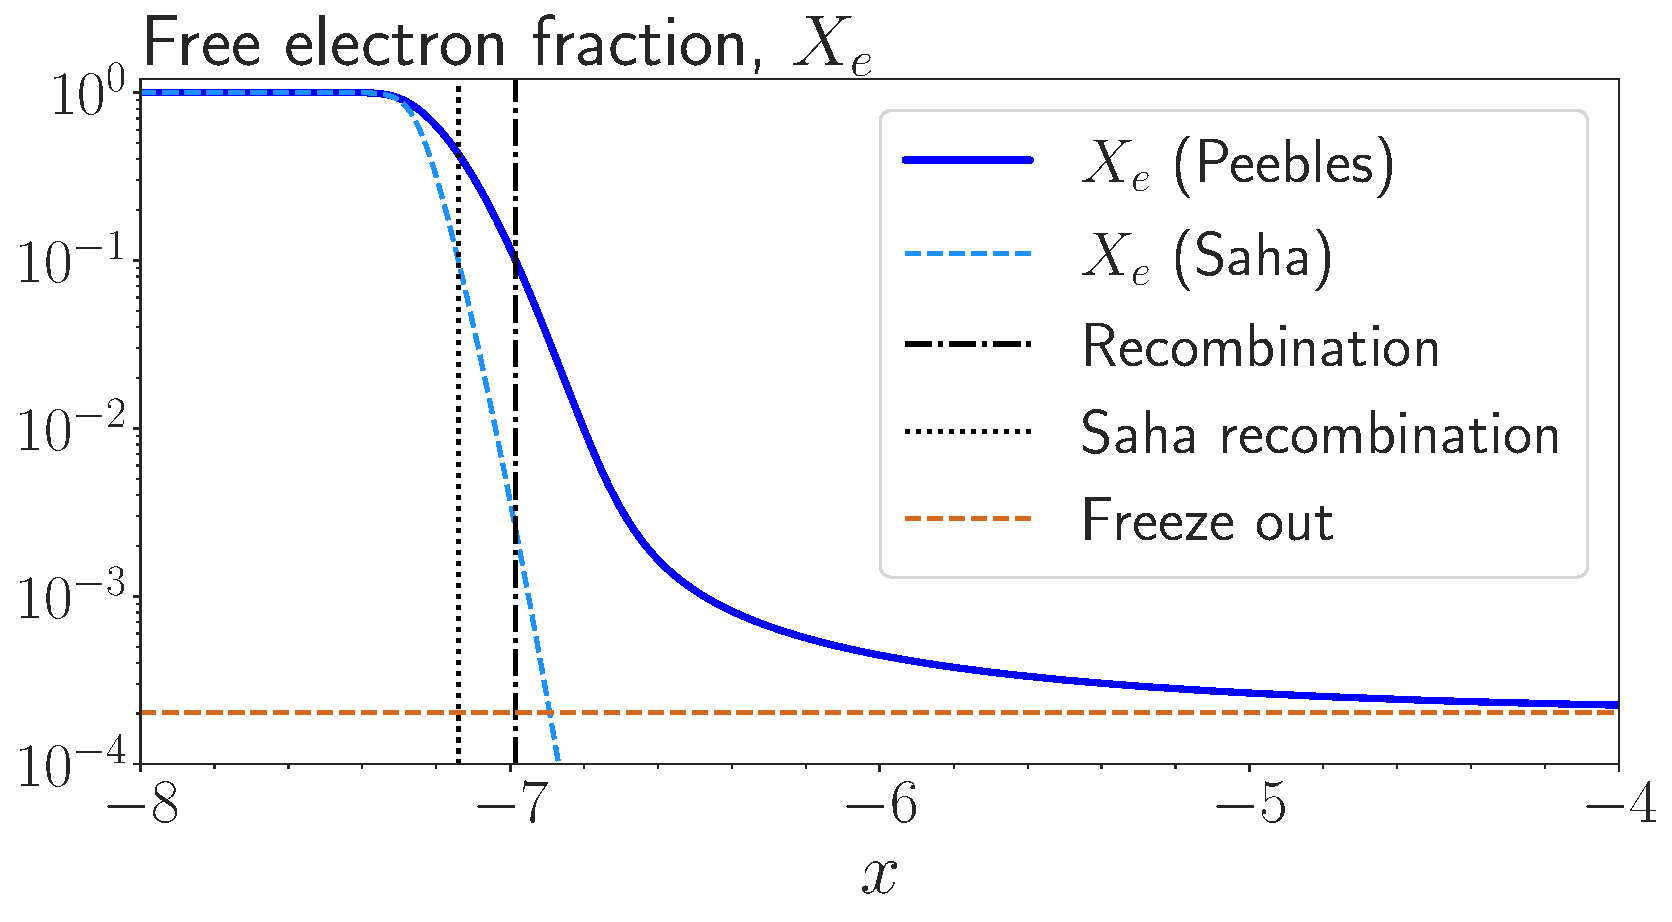
\includegraphics[width=\linewidth]{Xe_plot.pdf}
        \caption{Somecaption}
        \label{fig:m2:electron_fraction}
    \end{figure}

    \begin{figure}
        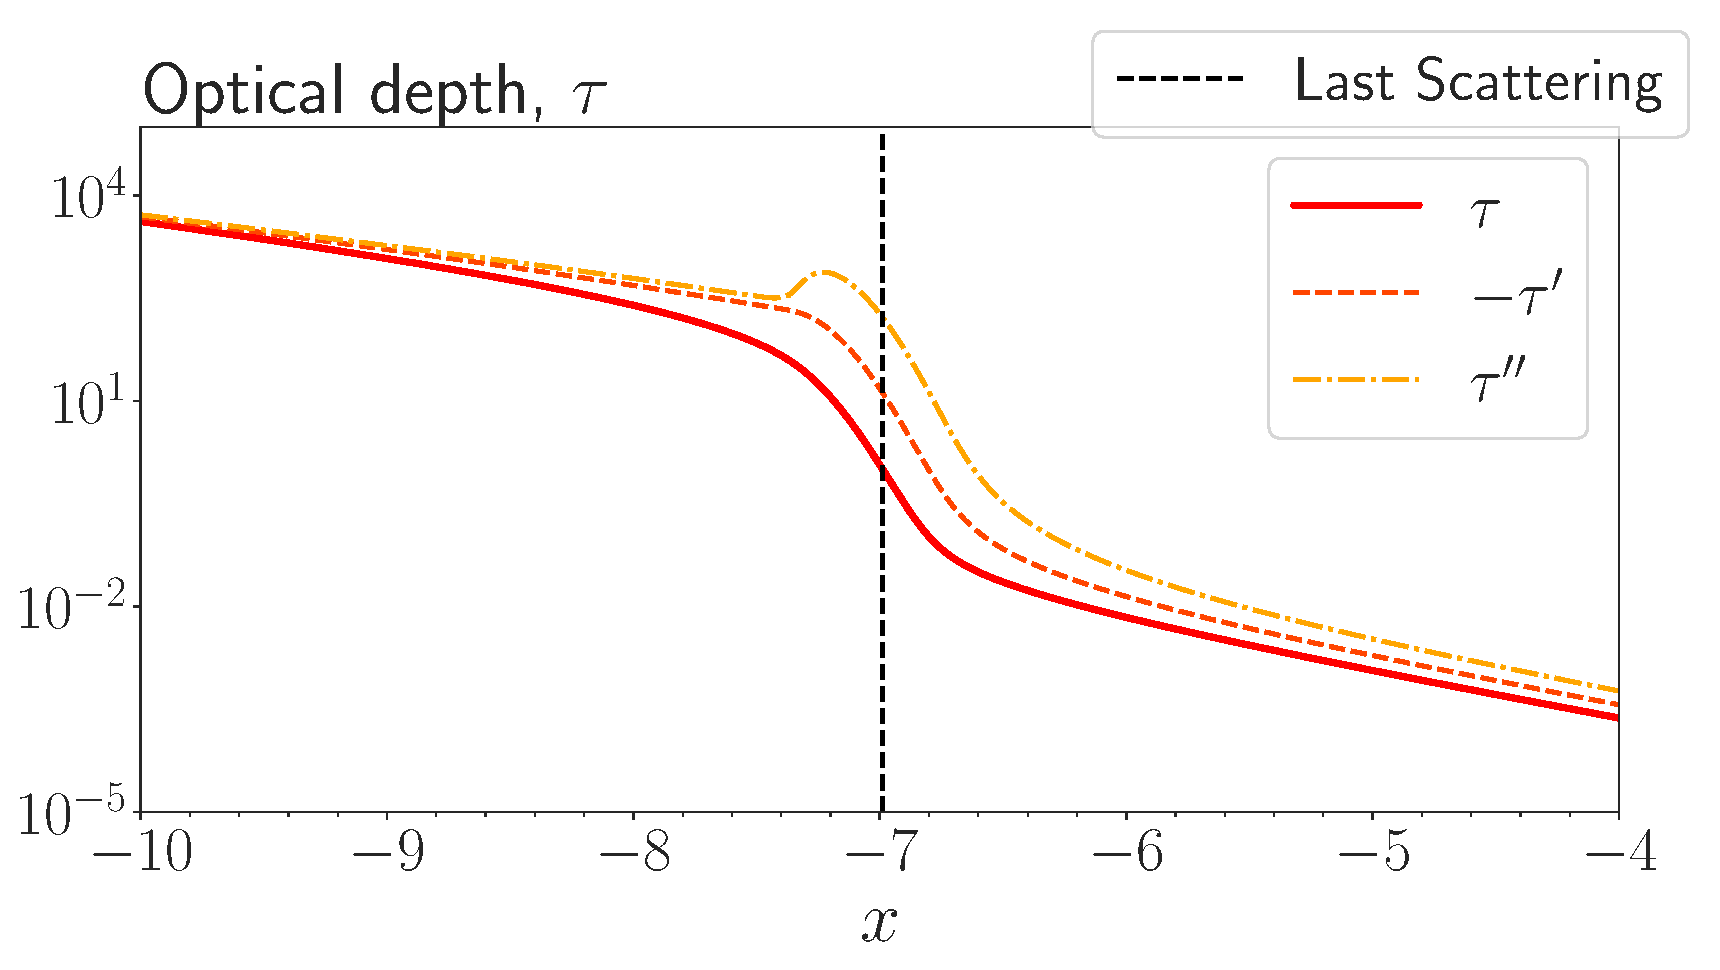
\includegraphics[width=\linewidth]{optical_depth.pdf}
        \caption{Somecaption}
        \label{fig:m2:optical_depth}
    \end{figure}

    \begin{figure}
        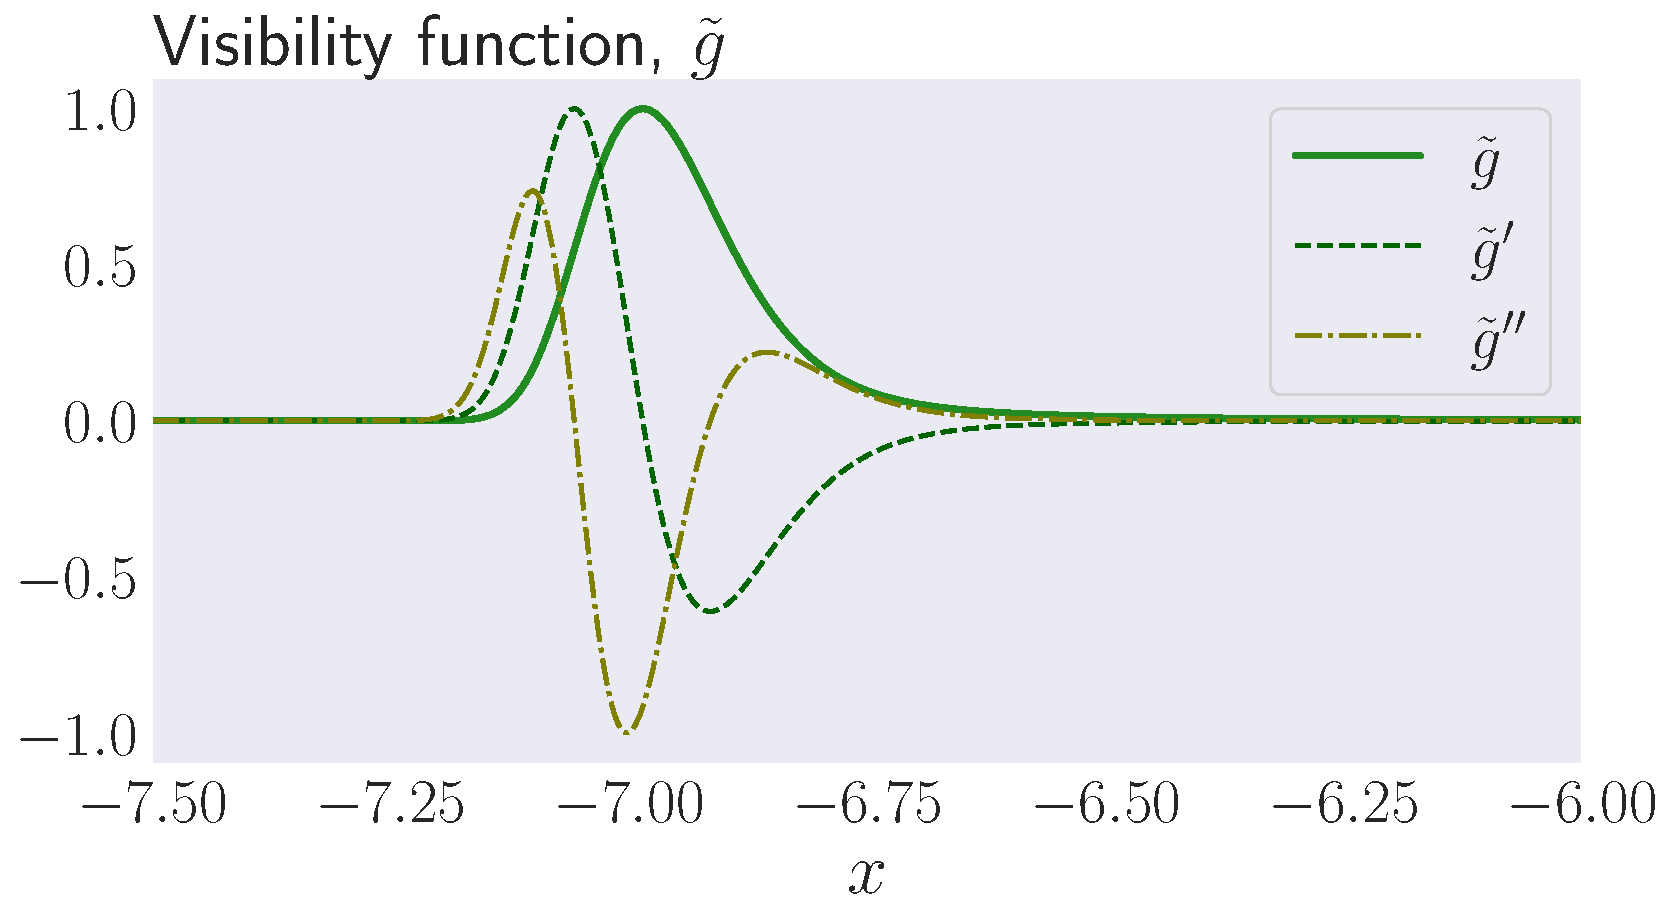
\includegraphics[width=\linewidth]{visibility_function.pdf}
        \caption{Somecaption}
        \label{fig:m2:visibility_function}
    \end{figure}

    % \begin{figure}
    %     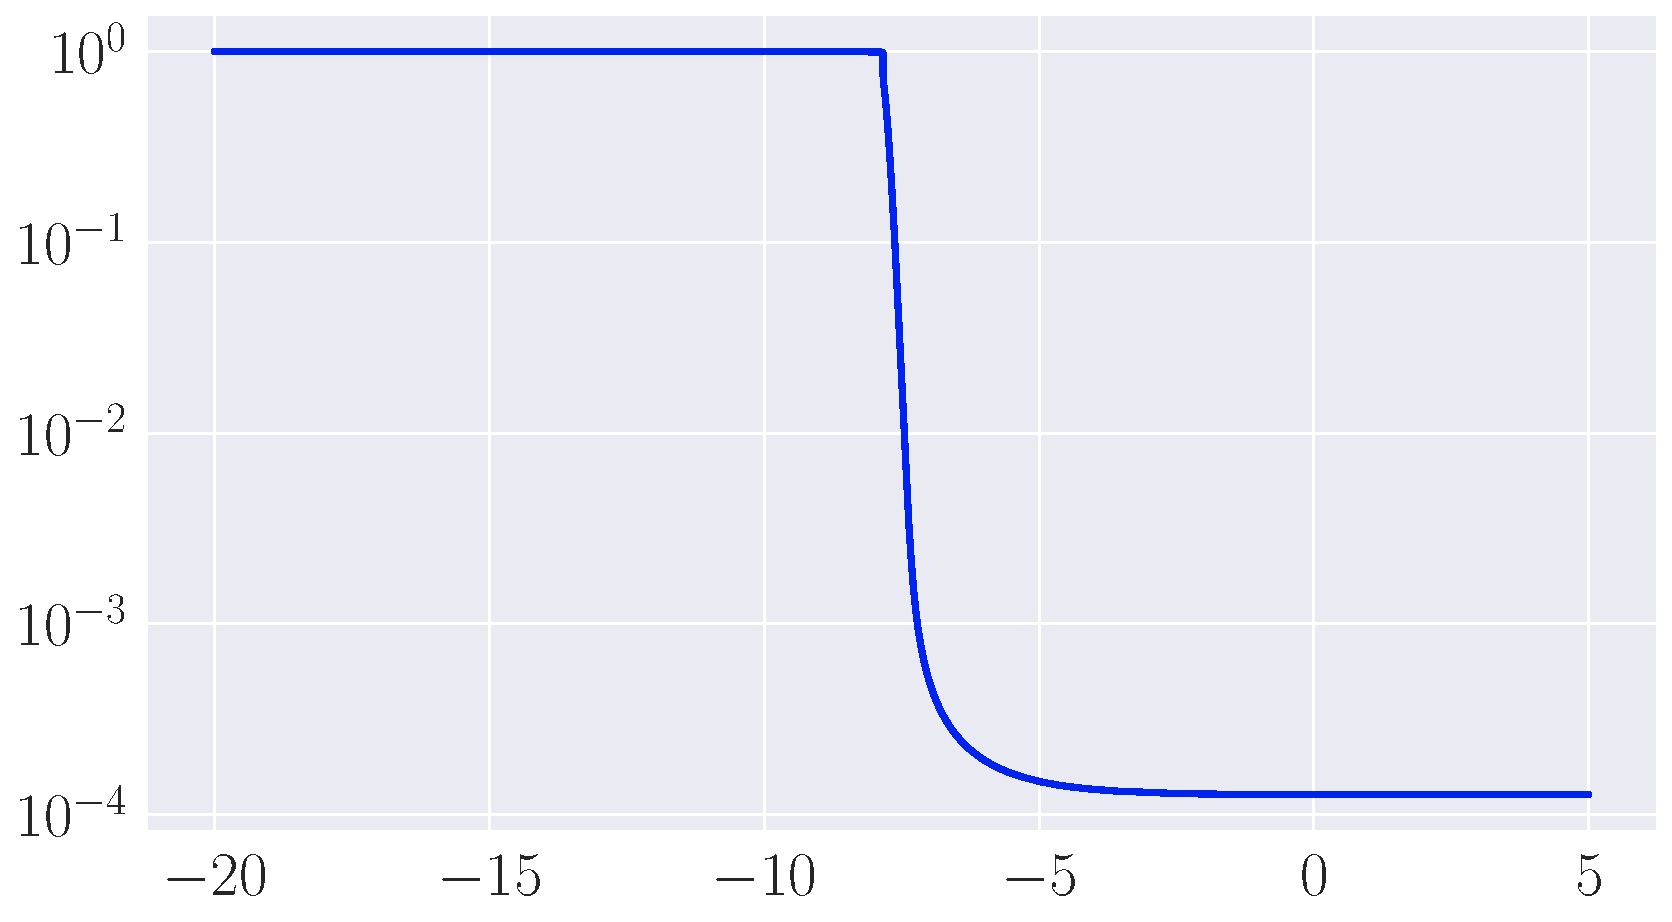
\includegraphics[width=\linewidth]{Xe_electron_fraction.pdf}
    %     \caption{SOMECAPTION Electron fraction}
    %     \label{fig:m2:electron_fraction_Xe}
    % \end{figure}


    % \begin{figure}
    %     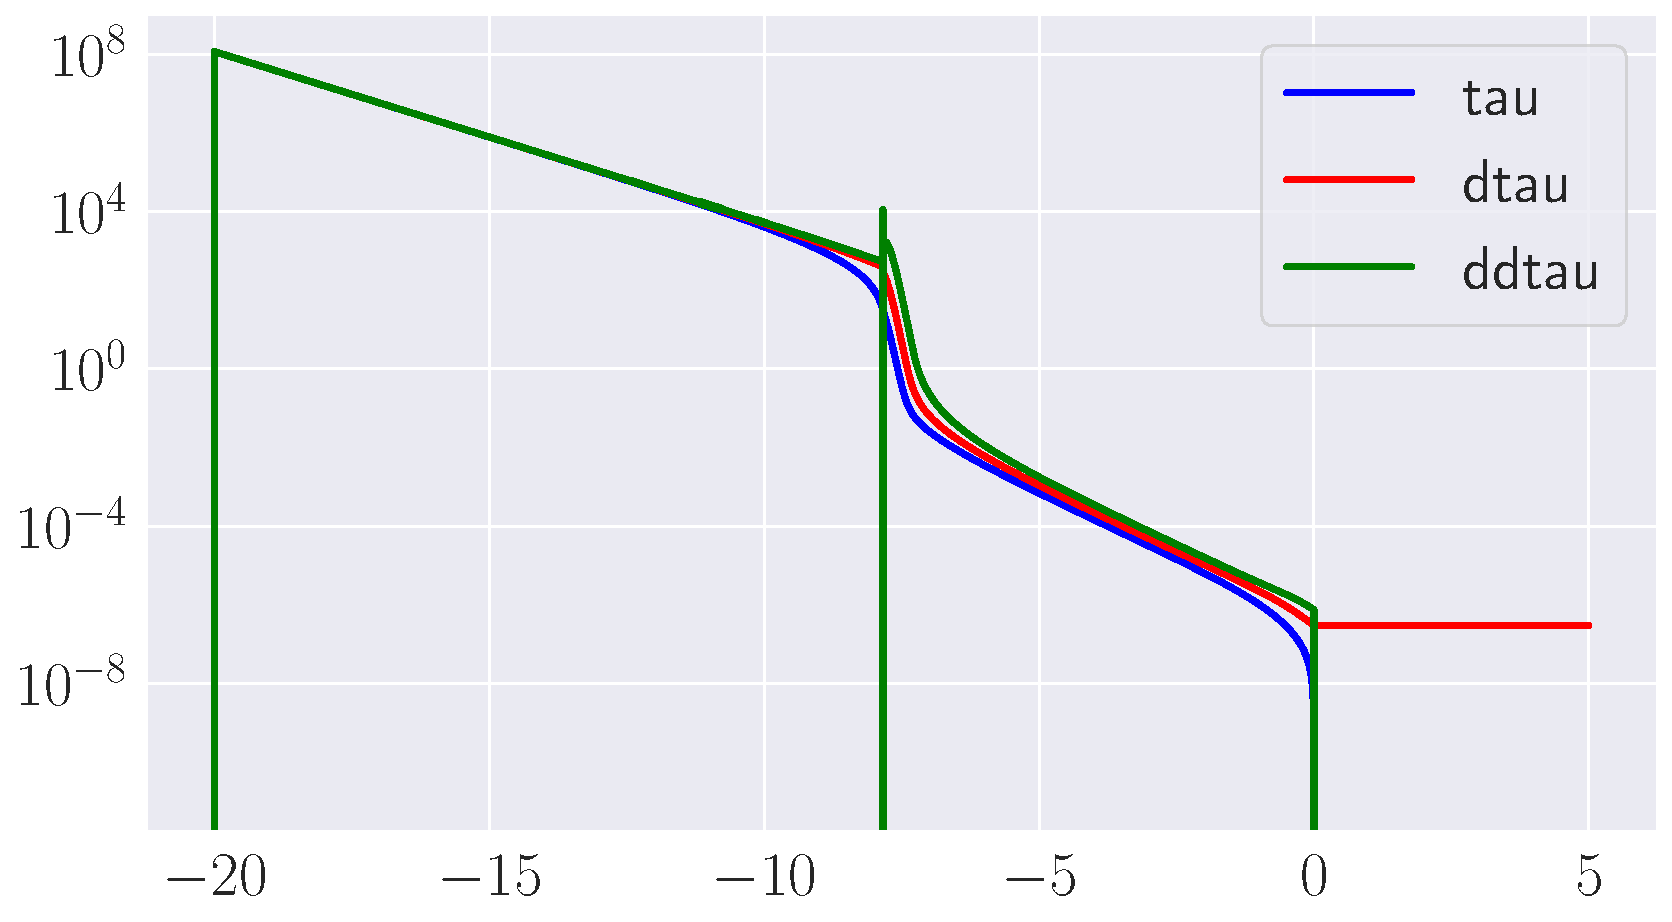
\includegraphics[width=\linewidth]{tau_of_x.pdf}
    %     \caption{SOMECAPTION tau of x}
    %     \label{fig:m2:tau_of_x}
    % \end{figure}


    % \begin{figure}
    %     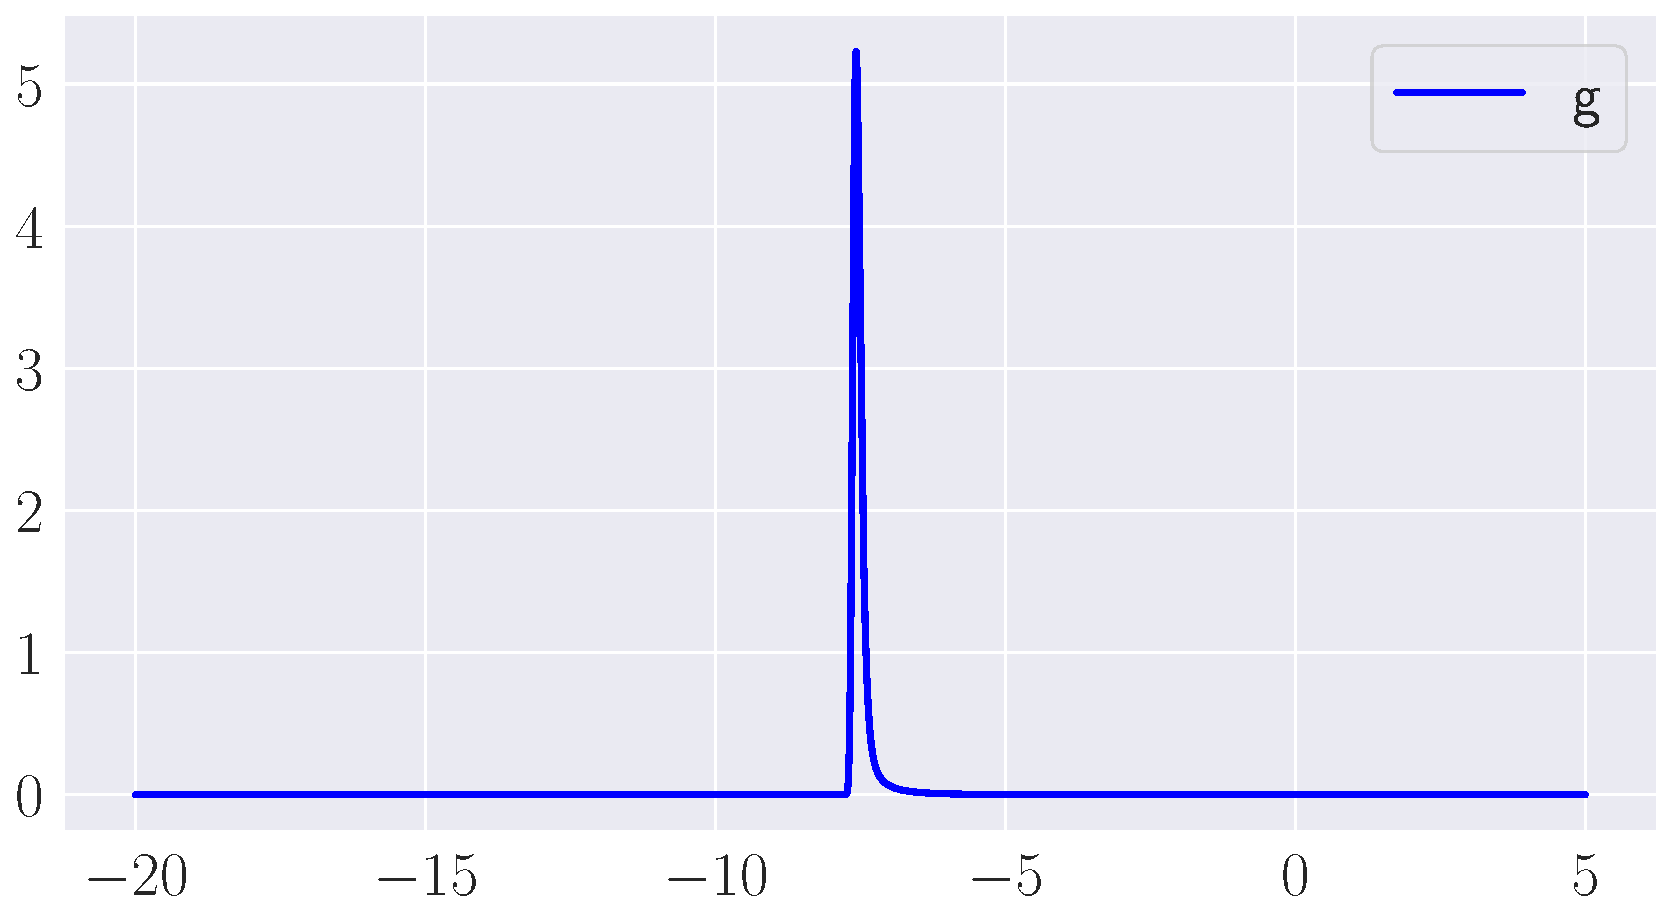
\includegraphics[width=\linewidth]{g_of_x.pdf}
    %     \caption{SOMECAPTION g of x}
    %     \label{fig:m2:g_of_x}
    % \end{figure}

    % \begin{figure}
    %     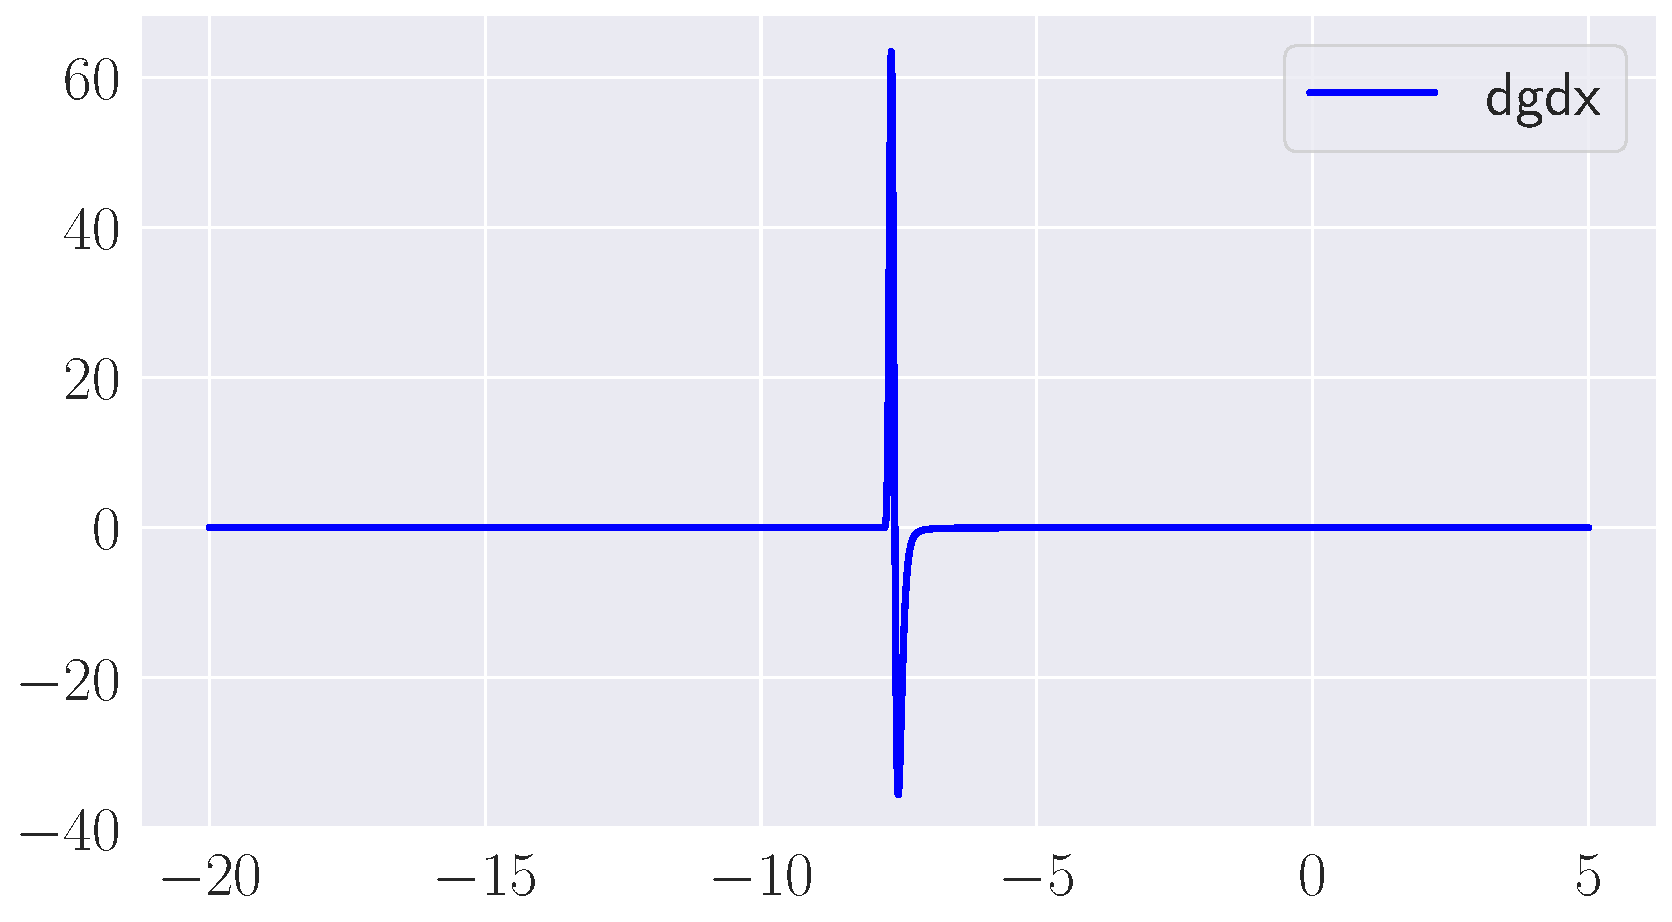
\includegraphics[width=\linewidth]{dg_of_x.pdf}
    %     \caption{SOMECAPTION dg of x}
    %     \label{fig:m2:dg_of_x}
    % \end{figure}

    % \begin{figure}
    %     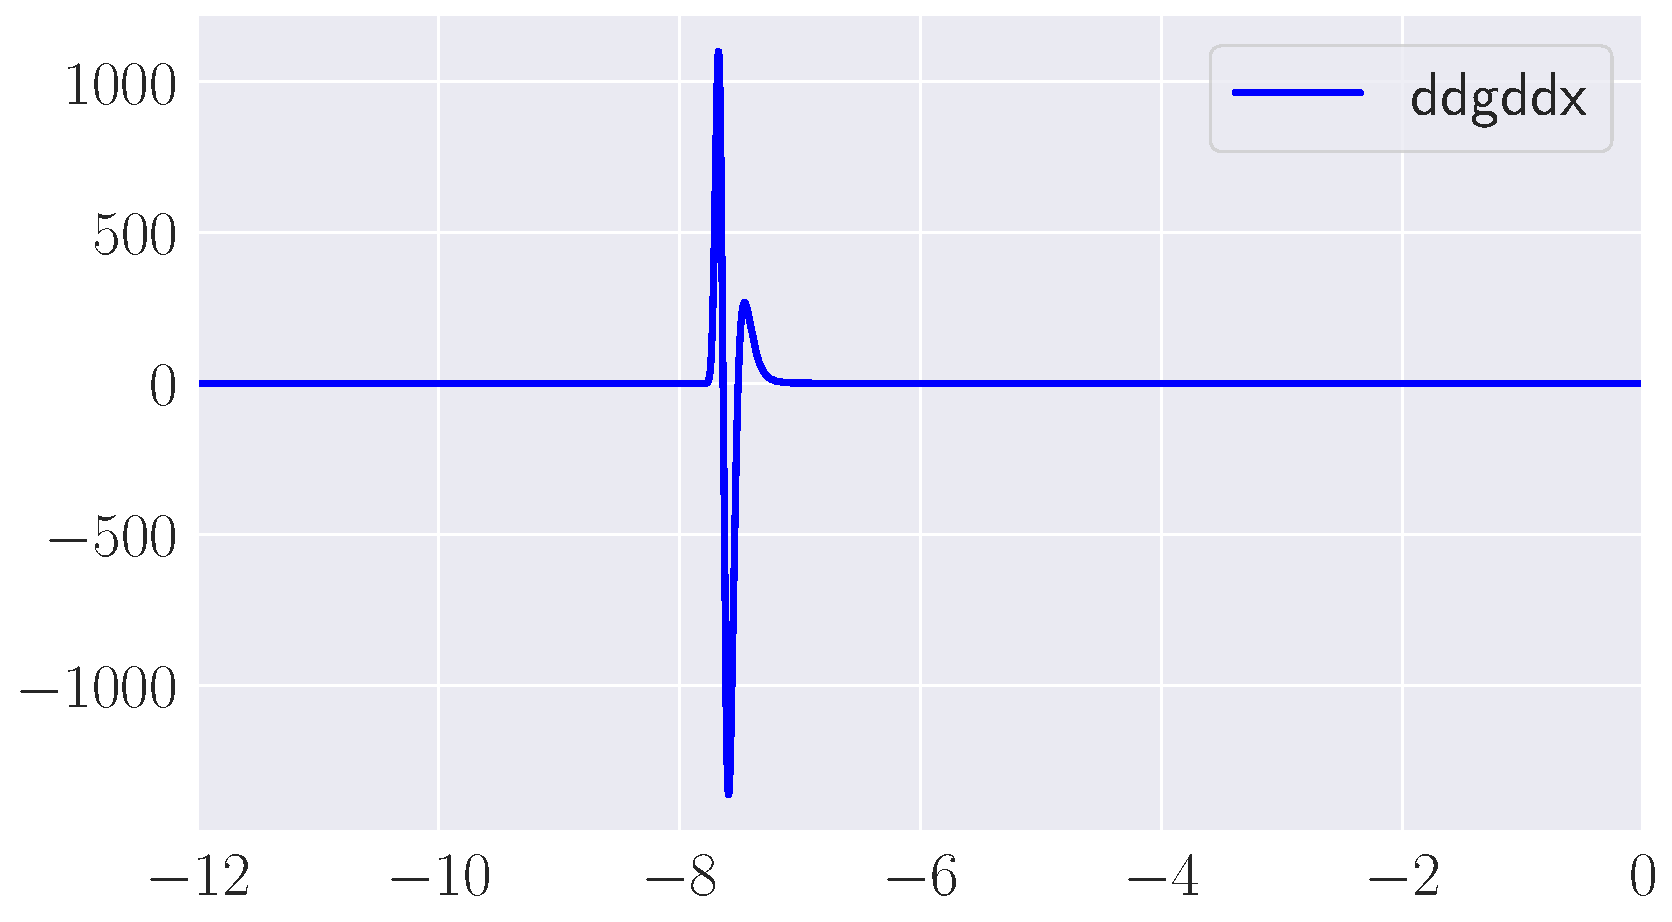
\includegraphics[width=\linewidth]{ddg_of_x.pdf}
    %     \caption{SOMECAPTION ddg of x}
    %     \label{fig:m2:ddg_of_x}
    % \end{figure}

